\documentclass[12pt]{article}
\title{\vspace{-2.5cm}\Large{Do Homeowners Care About Air Quality? Estimating the Effect of Poor Air Quality on Home Prices Using Wildfire Smoke Data}\\
{\large\textit{Model and Data}}} 
\author{\normalsize Tristan Misko}
\date{\normalsize{17 November 2021}}

\usepackage{amsmath}
\usepackage{amsfonts}
\usepackage{mathrsfs}
\usepackage{amssymb}
\usepackage{yfonts}
\usepackage{bbm}
\usepackage{graphics}
\usepackage[margin=1 in]{geometry}

\let\biconditional\longleftrightarrow
\let\iff\Leftrightarrow
\let\implies\Rightarrow
\let\infinity\infty
\let\by\times
\let\iso\cong
\let\unif\rightrightarrows
\DeclareRobustCommand{\Z}{\mathbb Z}
\DeclareRobustCommand{\hom}{\text{Hom}\,(\Z,G)}
\DeclareRobustCommand{\N}{\mathbb N}
\DeclareRobustCommand{\R}{\mathbb R}
\DeclareRobustCommand{\C}{\mathbb C}
\DeclareRobustCommand{\Q}{\mathbb Q}
\DeclareRobustCommand{\E}{\mathbb E}
\DeclareRobustCommand{\P}{\mathbb P}
\DeclareRobustCommand{\tr}{\text{tr}}
\DeclareRobustCommand{\norm}{\mathrel{\unlhd}}
\DeclareRobustCommand{\contains}{\supset}
\DeclareRobustCommand{\lcm}{\text{lcm}}
\DeclareRobustCommand{\glnr}{GL(n,\R)}
\DeclareRobustCommand{\limit}{\lim_{n\to\infinity}}
\DeclareRobustCommand{\nti}{{n\to\infinity}}
\DeclareRobustCommand{\del}{\partial}
\DeclareRobustCommand{\graph}{\text{graph}\,}
\DeclareRobustCommand{\interior}{\text{int}\,}
\DeclareRobustCommand{\Var}{\text{Var}}
\DeclareRobustCommand{\Cov}{\text{Cov}}
\DeclareRobustCommand{\normal}{\mathcal N}
\DeclareRobustCommand{\Bar}{\overline}

\usepackage{titlesec}
\titleformat*{\section}{\normalsize\bfseries}
\titleformat*{\subsection}{\normalsize\bfseries}
\titleformat*{\subsubsection}{\normalsize\bfseries}
\titleformat*{\paragraph}{\normalsize\bfseries}
\titleformat*{\subparagraph}{\large\bfseries}

\usepackage{mathtools}
\DeclarePairedDelimiter\ceil{\lceil}{\rceil}
\DeclarePairedDelimiter\floor{\lfloor}{\rfloor}
\usepackage{cancel}

\usepackage{pgfplots}
\usepackage{tikz}
\usetikzlibrary{patterns}
\usetikzlibrary{calc}
\usepgfplotslibrary{polar}

\usepackage[english]{babel}
\usepackage[utf8]{inputenc}
\usepackage{multicol}
\usepackage{fancyhdr}

\pagestyle{fancy}
\fancyhf{}
\lhead{Tristan Misko}
\rhead{\small{ECON 191}}
\cfoot{\thepage}

\usepackage{mathrsfs}
\usepackage{multirow}
\usepackage{hyperref}
\usepackage{textcomp}
\usepackage{xcolor}
\usepackage{setspace}

\usepackage{listings}
\usepackage{color}

\definecolor{dkgreen}{rgb}{0,0.6,0}
\definecolor{gray}{rgb}{0.5,0.5,0.5}
\definecolor{mauve}{rgb}{0.58,0,0.82}

\lstset{frame=tb,
  language=R,
  aboveskip=3mm,
  belowskip=3mm,
  showstringspaces=false,
  columns=flexible,
  basicstyle={\small\ttfamily},
  numbers=none,
  numberstyle=\tiny\color{gray},
  keywordstyle=\color{blue},
  commentstyle=\color{dkgreen},
  stringstyle=\color{mauve},
  breaklines=true,
  breakatwhitespace=true,
  tabsize=4
}

\begin{document}
	\maketitle
	\doublespacing
\vspace{-1.5cm}	
\section{Model and Design}

\begin{table}[!htbp] \centering 
  \caption{Effect of Wildfire Smoke on Housing Prices} 
  \label{} 
\begin{tabular}{@{\extracolsep{6pt}}lcc} 
\\\hline  \hline \\ 
\\ & (1) & (2)\\ 
\hline \\[-1.8ex] 
 (Intercept) & 183687.00$^{***}$ & 73976.901 \\ 
  & (1100.8998) & (1113.0914) \\ 
  & & \\ 
 n.score & $-$0.6631 &  \\ 
  & (0.6412) &   \\ 
  & &  \\ 
 treat.k5.t50 & & $-$1484.0340$^{***}$  \\ 
  & & (168.9167) \\ 
  & & \\ 
 unemp & 1114.7302$^{***}$ & 1563.9206$^{***}$  \\ 
  & (27.7190) & (48.1914)  \\ 
  & & \\ 
 County Fixed Effects& Yes & Yes  \\ 
  &  &    \\ 
 Time Fixed Effects & Yes & Yes \\ 
  &  &    \\ 
 
\hline \\[-1.8ex] 
Observations & 234600 & 45655 \\ 
R$^{2}$ & 0.9804 & 0.98367 \\ 
\hline 
\hline \\[-1.8ex]  \\ 
\end{tabular} 
\end{table} 

\begin{table}[!htbp] \centering 
  \caption{} 
  \label{} 
\begin{tabular}{@{\extracolsep{5pt}}lccccc} 
\\[-1.8ex]\hline 
\hline \\[-1.8ex] 
Statistic & \multicolumn{1}{c}{N} & \multicolumn{1}{c}{Mean} & \multicolumn{1}{c}{St. Dev.} & \multicolumn{1}{c}{Min} & \multicolumn{1}{c}{Max} \\ 
\hline \\[-1.8ex] 
X & 234,600 & 117,300.500 & 67,723.330 & 1 & 234,600 \\ 
year & 234,600 & 2,014.696 & 2.773 & 2,010 & 2,019 \\ 
month & 234,600 & 6.652 & 3.434 & 1 & 12 \\ 
zhvi.score & 234,600 & 135,041.500 & 79,504.160 & 22,372 & 1,646,548 \\ 
SizeRank & 234,600 & 1,328.630 & 787.017 & 1 & 3,071 \\ 
STATEFP & 234,600 & 32.497 & 13.459 & 10 & 55 \\ 
COUNTYFP & 234,600 & 114.463 & 117.166 & 1 & 840 \\ 
n.light & 234,600 & 2.748 & 4.662 & 0.000 & 30.714 \\ 
n.medium & 234,600 & 0.584 & 1.625 & 0.000 & 25.995 \\ 
n.heavy & 234,600 & 0.130 & 0.550 & 0 & 12 \\ 
n.score & 234,600 & 25.749 & 55.318 & 0.000 & 820.000 \\ 
period & 234,600 & 58.000 & 33.196 & 1 & 115 \\ 
unemp & 234,600 & 5.908 & 2.505 & 1.100 & 21.648 \\ 
post43 & 234,600 & 0.626 & 0.484 & 0 & 1 \\ 
post48 & 234,600 & 0.583 & 0.493 & 0 & 1 \\ 
post55 & 234,600 & 0.522 & 0.500 & 0 & 1 \\ 
post60 & 234,600 & 0.478 & 0.500 & 0 & 1 \\ 
post67 & 234,600 & 0.417 & 0.493 & 0 & 1 \\ 
m.s.pre43 & 234,600 & 28.083 & 15.841 & 5.602 & 61.858 \\ 
m.s.post43 & 234,600 & 24.355 & 15.515 & 2.782 & 75.967 \\ 
m.s.delta43 & 234,600 & $-$3.729 & 10.237 & $-$36.251 & 30.297 \\ 
m.s.pch43 & 234,600 & $-$0.059 & 0.403 & $-$0.820 & 1.634 \\ 
m.s.pre48 & 234,600 & 25.528 & 14.411 & 5.129 & 56.054 \\ 
m.s.post48 & 234,600 & 25.907 & 16.633 & 2.911 & 81.352 \\ 
m.s.delta48 & 234,600 & 0.378 & 10.704 & $-$31.451 & 39.691 \\ 
m.s.pch48 & 234,600 & 0.108 & 0.493 & $-$0.796 & 2.159 \\ 
m.s.pre55 & 234,600 & 26.099 & 14.801 & 4.814 & 60.081 \\ 
m.s.post55 & 234,600 & 25.428 & 15.898 & 2.941 & 79.808 \\ 
m.s.delta55 & 234,600 & $-$0.671 & 8.164 & $-$25.744 & 29.185 \\ 
m.s.pch55 & 234,600 & 0.031 & 0.338 & $-$0.754 & 1.295 \\ 
m.s.pre60 & 234,600 & 24.754 & 14.237 & 4.637 & 57.425 \\ 
m.s.post60 & 234,600 & 26.834 & 16.644 & 2.963 & 83.996 \\ 
m.s.delta60 & 234,600 & 2.081 & 8.551 & $-$22.197 & 34.476 \\ 
m.s.pch60 & 234,600 & 0.156 & 0.387 & $-$0.728 & 1.536 \\ 
m.s.pre67 & 234,600 & 26.489 & 15.616 & 4.153 & 66.977 \\ 
m.s.post67 & 234,600 & 24.716 & 14.460 & 3.395 & 74.525 \\ 
m.s.delta67 & 234,600 & $-$1.773 & 6.198 & $-$19.957 & 17.780 \\ 
m.s.pch67 & 234,600 & $-$0.012 & 0.265 & $-$0.683 & 0.992 \\ 
\hline \\[-1.8ex] 
\end{tabular} 
\end{table} 

The main idea of the paper is to determine whether housing prices respond to 
changes to in air quality.  The naive regression of housing prices on air quality
may suffer from significant endogeneity.  If homeowners respond to air quality, then
it is likely that taste-based sorting occurs, producing a selection bias.  To overcome endogeneity, we use wildfire smoke as a source of exogenous variation in
air quality and exploit the heterogeneous increase in wildfire smoke since 2015 to 
obtain casual estimates.

\section{Description of Data}

%\subsection{Summary of Data Structure}
The data take the form of panel data, with monthly observations at the county level
of the number of days in each month in which the county is covered by wildfire 
smoke plumes, the mean air quality index (AQI) over the month, and the level of 
the Zillow housing price index in that month.  I also have associated to each observation a set of controls for unemployment level and housing characteristics. 
The data range from June 2010 to July 2019 and contain counties outside of the
geographic west of the United States (such counties may suffer potentially
significant confounding from wildfires themselves).  I am currently working on 
expanding the smoke dataset to include all months in 2019 and 2020.

%\subsection{Smoke Data}

%The smoke data, in the form of dummies for exposure to light, medium, and heavy wildfire smoke, are reported by Vargo at the census block and daily level, so both spatial and temporal aggregation was necessary in order to bring the data up to the county and monthly level.  A number of nontrivial decisions were made in the aggregation process which require validation via robustness checks.  

%First, we grouped at the county level and computed a population-weighted "dummy" which takes values on the interval [0,1] for smoke exposure in each of the three intensity categories within a county on a given day.  For example, a value of 0.5 for the `light` would indicate that 50\% of the county's population was exposed to light wildfire smoke on a given day.

%We then aggregated to the monthly level by grouping observations by month and summing the population weighted county level smoke exposure indicators to obtain a ``number'' of days of smoke exposure at the light, medium, and heavy levels.  This number is continuously valued because of the above weighting scheme but is bounded by the number of days in the month.

% Finally, we summarize across the light, medium, and heavy levels by computing the variable smoke$\_$score.  There is a fairly natural weighting scheme for aggregation.  NOAA defines plumes with density 0-10 $\mu g/m^3$ as light, 10-21 $\mu g/m^3$ as medium, and $>22\mu g/m^3$ as heavy, so computing the weighted sum 
%$$\text{smoke\_score} = 5*\text{light} + 15*\text{medium} + 25*\text{heavy}$$ 
%gives a rough measure of the total density of smoke exposure over a given month for a given county.

\section{Empirical Strategy}

A county is categorized as treated if the difference between its post-2014 monthly mean smoke 
score and its pre-2014 monthly mean smoke score is greater than some threshold value $\alpha$.
Likewise, control counties are determined by finding those counties whose difference is less
than some threshold $\beta$.  This leaves a group of ``boundary'' counties which are neither
treatment nor control counties.  The coefficient of interest is $\delta$, which we expect to be small and to have a negative sign.  This basic model is given by \begin{singlespace}$$\text{price}_{c,t} = \delta\cdot\text{smoke}_{c,t}+ D_c + T_t +\gamma\cdot\text{Unemp}_{c,g(t)} + \zeta\cdot\text{HC}_{c,t} + \epsilon_{c,t}. $$

\textbf{Variable Descriptions:}

\begin{itemize}
\item $\text{price}_{c,t}$ (\textit{numeric variable}): The Zillow Home Value Index 
value, a smoothed indicator of housing prices in county $d$ and time period $t$.
\item $\text{smoke}_{c,t}$ (\textit{dummy variable}): A time-dependent treatment variable
determined from the smoke score, which a weighted sum of the number of light, medium
and heavy smoke days over the month within each county.  The dummy is one if we are in the
post treatment period (beginning 2015) and the county
experiences a change in mean monthly smoke score above a threshold value across the pre- and post-treatment period.
\item $D_c$ (\textit{dummy variable}): A set of dummy variables for the county fixed effects.  
\item $T_t$ (\textit{dummy variable}): A set of dummy variables for the time fixed  effects.
\item $\text{Unemp}_{c,g(t)}$ (\textit{numeric variable}): The quarterly unemployment rate at the county level.  Here, $g$ denotes the mapping of months to quarters.  
\item $HC_{c,t}$ (\textit{numeric variable}): A set of controls for the characteristics of the average home in a county
\end{itemize}
\end{singlespace}

\subsection{Further Models}
One extension that I am still setting up is the instrumental variables model,
which uses smoke treatment level instrument for Air Quality Index (AQI) in the 
first stage model, then estimates the causal effect of air quality on housing
prices in the second stage model.  

Since my treatment variable has differing dosage levels, I am looking into the 
literature on estimating Two-Way Fixed Effects models to employ on my data.  For now, I will
estimate some extensions of the basic model, I will use multiple dummies encoding different buckets of smoke score values.  See the below for a discussion of robustness checks of these arbitrary threshold values.

\subsection{Robustness Checks}
There are a number of robustness checks that remain to be done for my paper.  The
first and most important will be parallel trends in ZHVI for the difference-in-differences
estimation strategy.  Checking that ZHVI trends do not differ significantly before treatment
is crucial for the estimates to be unbiased.  Robustness to perturbing the time of treatment
activation will also be checked.

The basic model also depends on the selection of threshold values for the smoke score difference to determine inclusion in the treatment or control group.  The regression estimates will be recorded in graphs in which these threshold values are varied continuously to demonstrate the sensitivity of the results to the thresholds.  In addition, we will reestimate all equations using different weights within the aggregation scheme of the smoke dataset to ensure that the final results are not sensitive to weighting decisions.

\section{Data Summary Table}

The summary statistics for the main data are displayed in the table below. The variable \lstinline{zhvi.score} encodes housing prices. The variables \lstinline{n.light}, \lstinline{n.medium}, and \lstinline{n.heavy} encode the number of smoke days in the month at a given smoke intensity.  \lstinline{n.score} records the smoke score.  The control datasets are still being cleaned and processed, so they have not yet been matched to the main data frame, but I do have the .csv files on my machine.  

\begin{table}[!htbp] \centering 
  \caption{Summary Statistics of Main Variables} 
  \label{} 
\begin{tabular}{@{\extracolsep{5pt}}lcccccc} 
\\[-1.8ex]\hline 
\hline \\[-1.8ex] 
Statistic & \multicolumn{1}{c}{N} & \multicolumn{1}{c}{Mean} & \multicolumn{1}{c}{St. Dev.} & \multicolumn{1}{c}{Min} & \multicolumn{1}{c}{Median} & \multicolumn{1}{c}{Max} \\ 
\hline \\[-1.8ex] 
zhvi.score & 234,600 & 135,041.500 & 79,504.160 & 22,372 & 115,794 & 1,646,548 \\ 
n.light & 234,600 & 2.748 & 4.662 & 0.000 & 0.316 & 30.714 \\ 
n.medium & 234,600 & 0.584 & 1.625 & 0.000 & 0.000 & 25.995 \\ 
n.heavy & 234,600 & 0.130 & 0.550 & 0 & 0 & 12 \\ 
n.score & 234,600 & 25.749 & 55.318 & 0.000 & 1.671 & 820.000 \\ 
period & 234,600 & 58.000 & 33.196 & 1 & 58 & 115 \\ 
post2014 & 234,600 & 0.522 & 0.500 & 0 & 1 & 1 \\ 
\hline \\[-1.8ex] 
\end{tabular} 
\end{table}

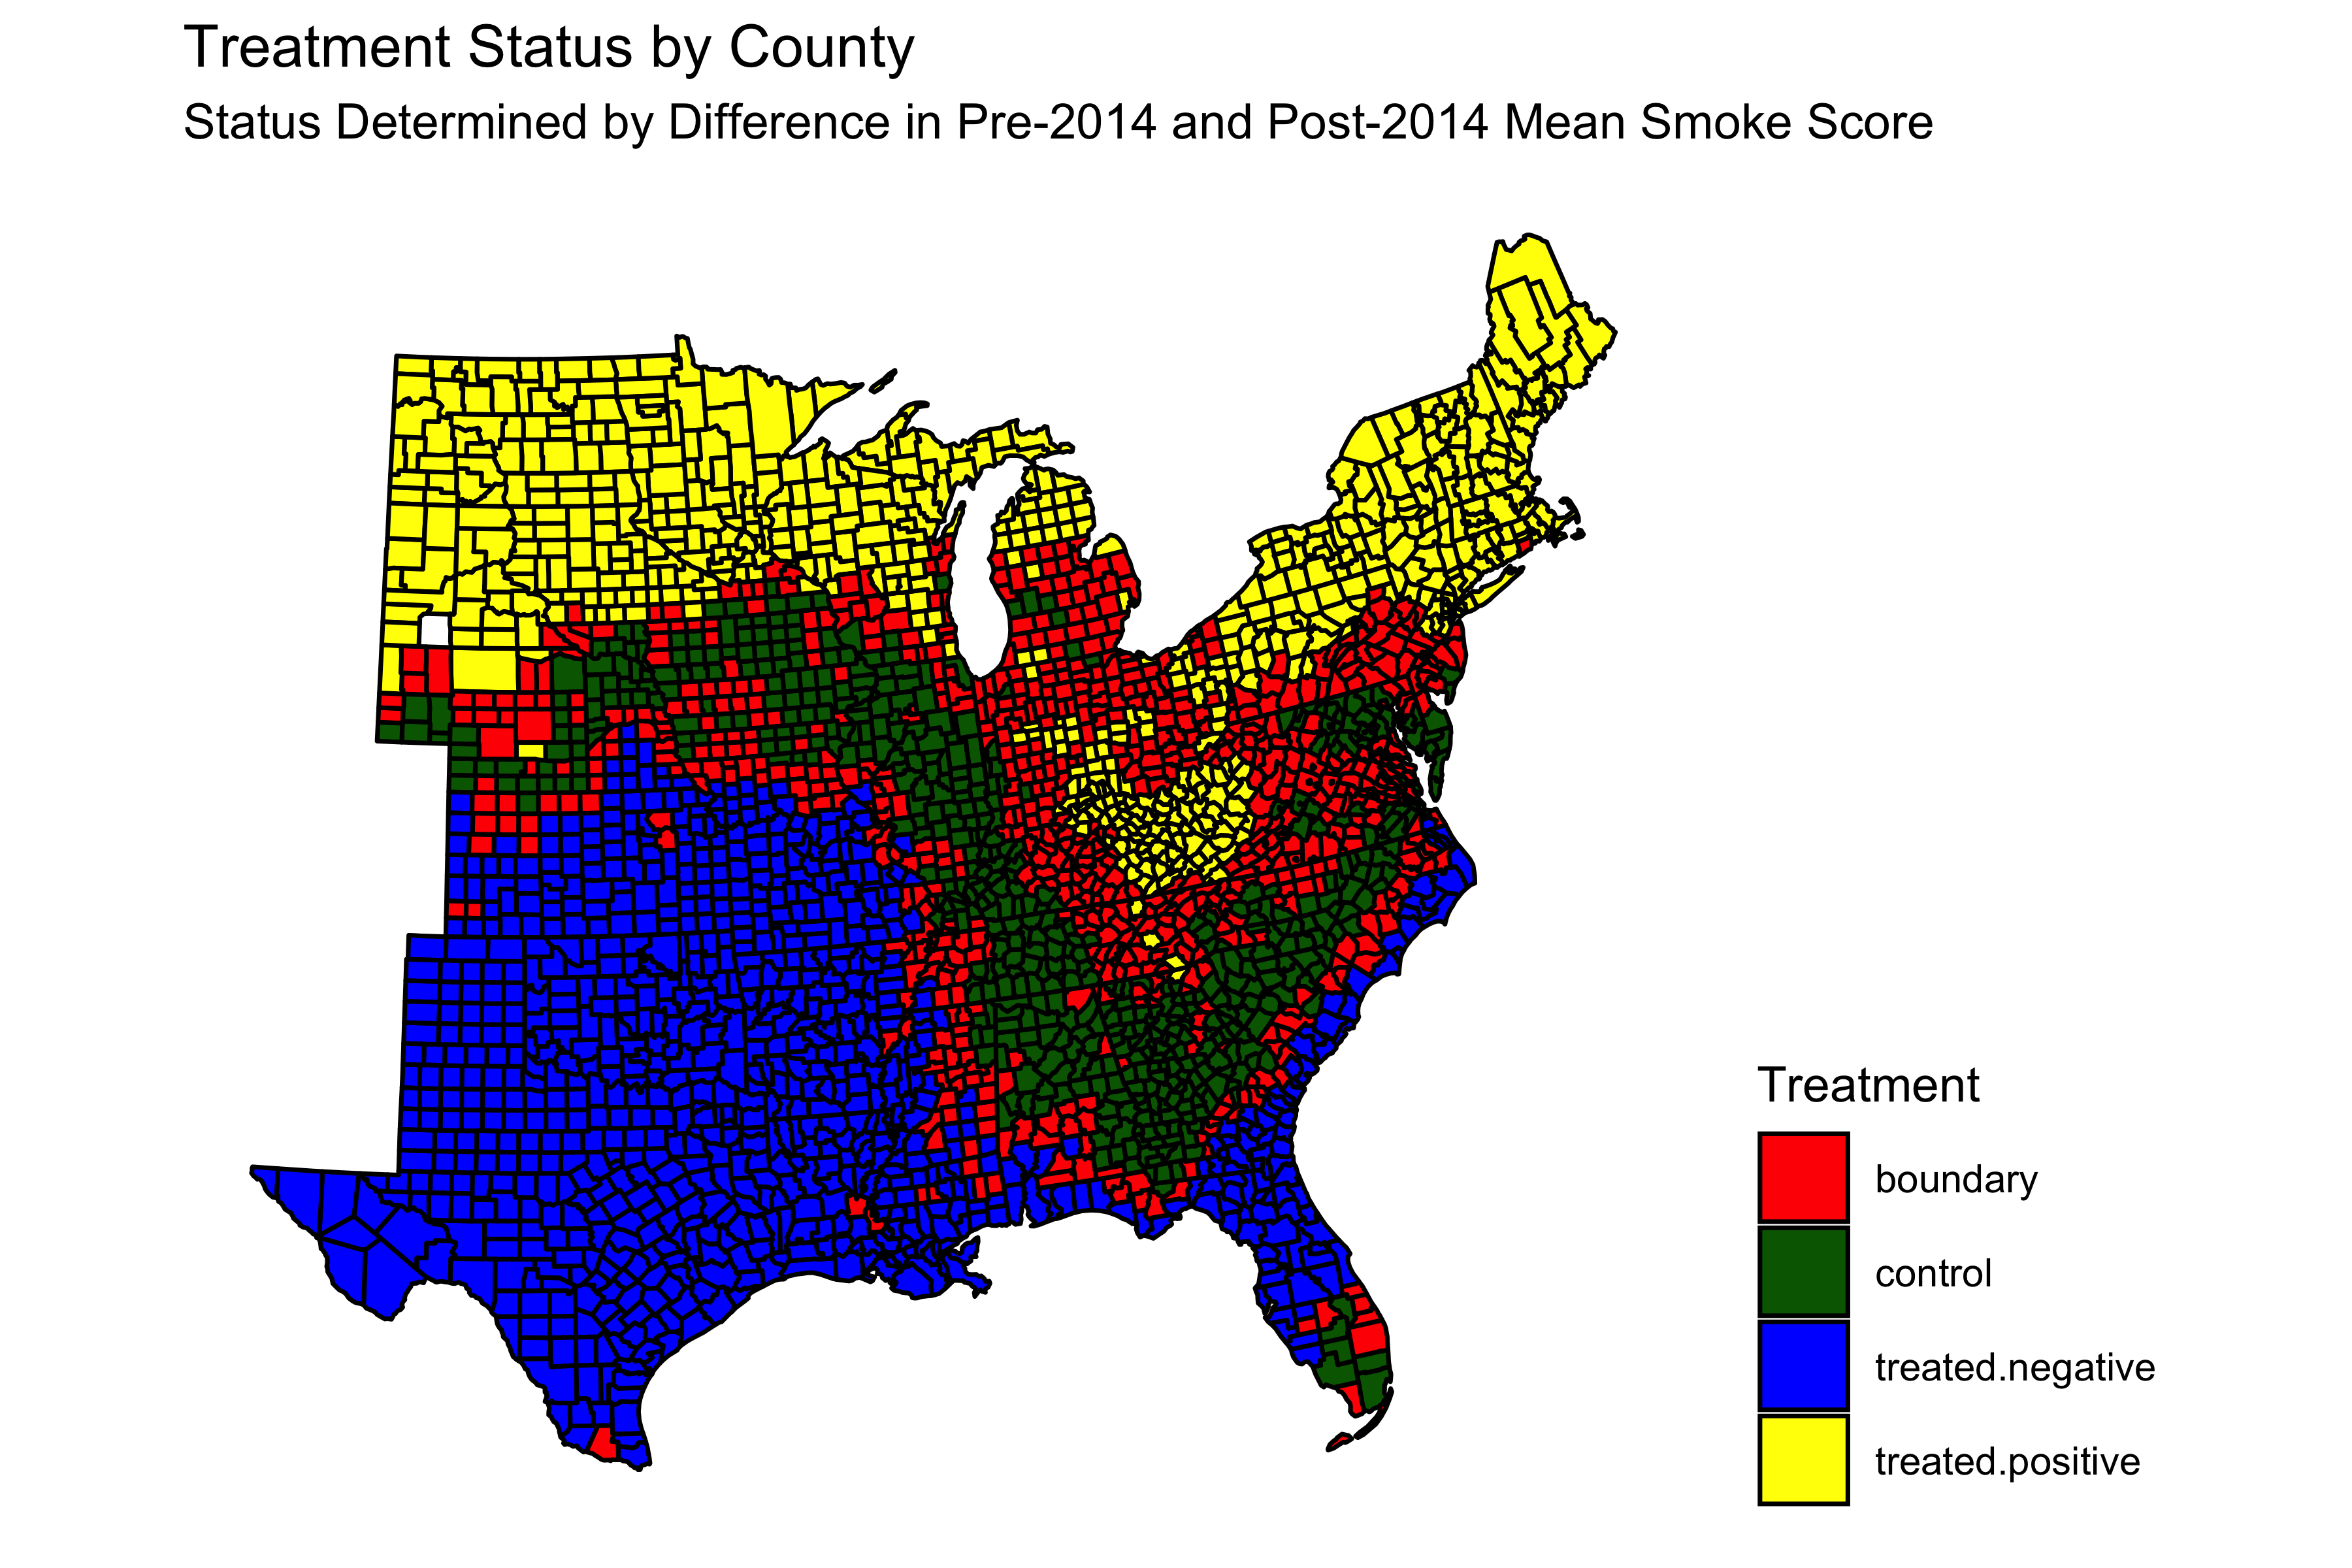
\includegraphics[scale = 0.15]{transparent}

\end{document}